\chapter{EV model and synthetic dataset}
\label{sec:ev_model_ds_gen}

In order to train a machine learning regression model for estimating the SOH of an EV battery pack, it is critical to have a relatively large dataset of EV monitoring data to use for training. However, as of today, the availability of large-scale, freely accessible datasets of real EV monitoring data is very limited \cite{ev_no_real_datasets}.

To overcome this issue, we may generate the required dataset synthetically.

The first step is to develop a mathematical model of an electric vehicle (sec. \ref{sec:ev_model}). The model must fulfil the following requirements:
\begin{itemize}
    \item it should capture and mimic with high accuracy the mechanical dynamics of a real EV in driving conditions (speed, motor torque, braking force, etc.), as well as the electro-thermal dynamics of the vehicle's battery pack (current, voltage, SOC, temperature, etc.). % accuracy
    \item it should be flexible enough to mimic a wide variety of real EVs just by changing its main mechanical/electrical parameters (so as to match those of the desired EV model). % flexibility
    \item the user can simulate the model upon specifying a driving cycle, external temperature, initial battery temperature, initial battery SOC, battery age (SOH). % user interaction
    \item the computational cost of performing a simulation should be reasonably low. % computational cost
\end{itemize}

The model can be used after its definition (sec. \ref{sec:ev_model}) and parametrization (sec. \ref{sec:model_parametrization}) to simulate an EV in different driving conditions and then collect the physical signals generated by multiple simulations to build a synthetic dataset of EV monitoring data (sec. \ref{sec:ds_gen}).





\section{EV Simulink model}
\label{sec:ev_model}
A simple electric vehicle model fulfilling all the requirements has been built through MATLAB\textsuperscript\textregistered and Simulink\textsuperscript\textregistered programming environments.
Similarly to a real vehicle, it is composed of many mutually dependent subsystems (such as the electric motor, battery pack, wheels, brakes, and so on), connected to each other through signals that are calculated and updated at each time step of the simulation. A visual representation of the EV model is shown in fig. \ref{fig:ev_model} in appendix \ref{appendix}.

This design is heavily based on an existing model found on MATLAB File Exchange \cite{racing_lounge}, but many components have been modified and improved to better suit our experimental needs, most notably the battery pack and the braking subsystem. A brief technical description of each component of the model is given in this section. Variable names which are written with the \texttt{typewriter} font are user-defined parameters of the vehicle.



\subsection{Driver}
\label{sec:driver}
This subsystem implements a discrete-time proportional-integral (PI) controller to mimic a human driver for the vehicle. At each time step the controller tracks the input reference speed (e.g. driving cycle speed signal) and the current simulated vehicle speed, and tries to match them by acting on the brake and accelerator pedals. Brake pedal position (\textit{BPP}) and accelerator pedal position (\textit{APP}) take values in the range $[0,1]$, where 0 stands for "not pressed" and 1 for "fully pressed".



\subsection{Motor}
\label{sec:motor}
The electric traction motor is used for propelling the EV. It is powered by electricity (supplied by the battery pack) and generates the power to rotate the wheels of the vehicle. Many types of electric motors exist; the main distinction is between DC and AC motors, depending on the type of electric flow they require to operate. Nowadays, most EVs feature an AC motor \cite{renault_motors}, either asynchronous (high power output) or synchronous (high torque output). Such EVs feature a DC/AC inverter to convert the DC supplied by the battery pack to the AC required to operate the AC motor (fig. \ref{fig:ev_powertrain}).
\begin{figure}[htb]
    \centering
    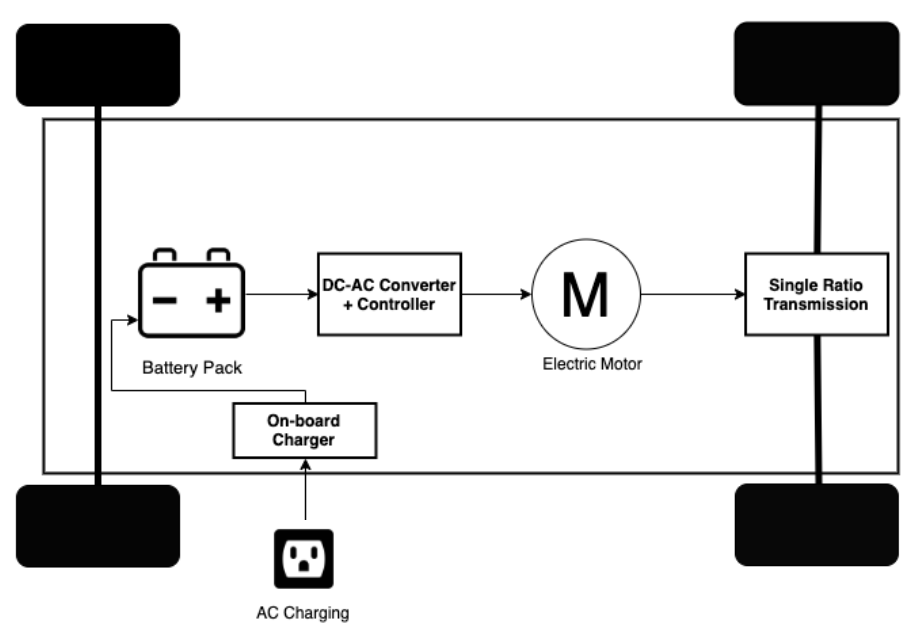
\includegraphics[width=0.7\textwidth]{images/ev_powertrain}
    \caption[Electrical powertrain of an EV]{Typical electrical powertrain of an EV equipped with an AC motor. Adapted from \cite{ev_reporter_powertrain}}
    \label{fig:ev_powertrain}
\end{figure}

Luckily, there exist a very simple characterization of an electric motor which is agnostic to its type and which is therefore used in our EV model \cite{hayes_ev_book}. Every electric motor can be characterized by two modes:
\begin{enumerate}
    \item Constant-torque mode: the motor can output a constant rated rotor torque, $T_{r(rated)}$, and the rotor power $P_r$ increases linearly with rotor/vehicle speed; achieved at low speeds.
    \item Constant-power mode: the motor can output a constant rated rotor power, $P_{r(rated)}$, and the rotor torque $T_r$ decreases inversely with rotor/vehicle speed; achieved at high speeds.
\end{enumerate}
This characterization is schematized in fig. \ref{fig:motor_characterization}.

\begin{figure}[htb]
    \centering
    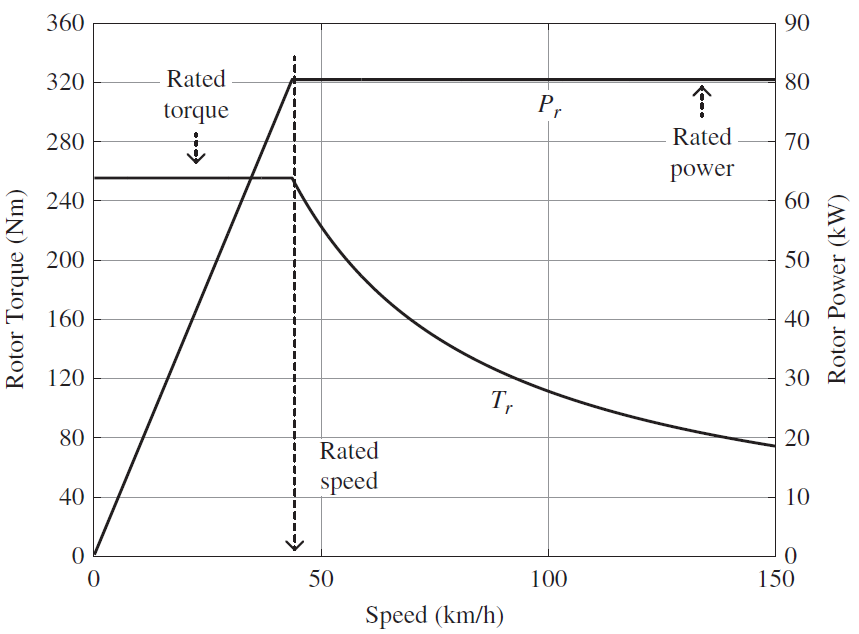
\includegraphics[width=0.7\textwidth]{images/motor_characterization}
    \caption[Torque-speed and power-speed envelopes]{Torque-speed and power-speed characterization curves for the electric motor of a 2015 Nissan Leaf. Taken from \cite{hayes_ev_book}}.
    \label{fig:motor_characterization}
\end{figure}

Moreover, there is a mathematical relation between power and torque
\begin{equation}
    P_r = T_r\omega_r = T_r \frac{v n_g}{r}
\end{equation}
where $\omega_r$ is the rotor speed [rad/s], $v$ is the vehicle speed [m/s], $n_g$ is the vehicle total drive ratio, $r$ is the radius of the wheels [m]. This means that we can characterize an electric motor just by specifying its torque-speed envelope.

On a final note, electric motors cannot convert 100\% of the electric power supplied by the battery ($P_{batt}$) to mechanical power, due to electrical and mechanical losses ($P_{losses}$) intrinsic to how the engine is designed. Losses are accounted for by introducing an efficiency term $\eta_{motor}$, so that the following equation holds:
\begin{equation}
P_r = P_{batt} - P_{losses} = \eta_{motor} P_{batt}
\end{equation}

We implement an electric motor in our EV model through the Mapped Motor block in Simulink \cite{mathworks:mapped_motor}. It is a mathematical model of an electric motor operated in torque-control mode. It can be parametrized by the user specifying a torque-speed envelope and other efficiency-related parameters:
\begin{itemize}
    \item \texttt{motorSpdRPM}: a vector of $N$ rotor speed values (in RPM), at which the value of maximum rotor torque is known
    \item \texttt{motorMaxTrq}: a vector of $N$ maximum rotor torque values [N$\cdot$m] which can be generated by the motor at a certain speed.
    \item \texttt{motorEff}: motor efficiency $\eta_{motor}$ at a rotor speed of \texttt{motorEffSpd} and a rotor torque of \texttt{motorEffTrq}
    \item \texttt{motorEffSpd}: rotor speed at which efficiency is measured [RPM]
    \item \texttt{motorEffTrq}: rotor torque at which efficiency is measured [N$\cdot$m]
    \item \texttt{motorPIron}: iron losses at the speed and torque at which efficiency is defined [W]
    \item \texttt{motorPBase}: fixed losses independent from torque and speed [W]
\end{itemize}

When the driver presses the accelerator pedal (i.e. $\text{APP}>0$), the model controls the mapped motor block with a rotor torque request of $\text{APP}\cdot T_{r(max)}(v)$. The block reads the current battery pack voltage $V_{batt}$, current rotor speed $\omega_r$ and the torque reference demand and computes the new rotor torque and the current $I_{batt}=P_{batt}/V_{batt}$ to be drawn from the battery to supply the needed power $P_r$.



\subsection{Braking system}
\label{sec:braking}
The braking system of an EV is based on two different contributes: friction braking and regenerative braking \cite{hayes_ev_book}.
The BPP value is interpreted as the fraction of the maximum total braking torque (\texttt{brqTrqMax}) that can be exerted on each wheel by the combination of friction and regenerative braking. The resulting braking torque "requested" by the driver is then distributed between the two braking subsystems, in such a way that the regenerative braking is used with priority and whenever possible, and friction braking only makes up for the remaining torque which cannot be supplied by regenerative braking. In formula:
\[
T_{braking} = \text{BPP} \cdot \text{\texttt{brqTrqMax}} = T_{regen} + T_{disc}
\]
The details about this distribution rule, known as brake blending \cite{brake_blending}, are discussed in the following paragraphs.

\paragraph{Regenerative braking}
Regenerative braking is a braking technology which achieves the aim of slowing down a vehicle while recharging its battery pack at the same time.
When the regenerative braking system is activated, the traction motor can develop a negative torque, up to the rated value in the forward direction. This torque reverses the usual flow of power such that the kinetic energy of the vehicle is converted to negative mechanical power on the driveshaft, and then converted to electrical power by the system. The generated electrical power is used to recharge the battery pack. This mechanism is schematized in fig. \ref{fig:regen_braking}.

\begin{figure}[htb]
    \centering
    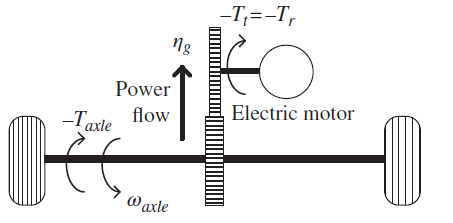
\includegraphics[width=0.6\textwidth]{images/regen_braking}
    \caption[Regenerative braking]{Regenerative braking scheme. Taken from \cite{hayes_ev_book}}.
    \label{fig:regen_braking}
\end{figure}

Recent studies \cite{regen_braking_limitations, wiki:regen_braking} suggest that regenerative braking is not energy-efficient nor sufficiently effective to apply at low speeds. For this reason, our model implements a user-defined cutoff speed (\texttt{RegenBrkSpd\_bpt}) above which the regenerative braking can be used. This is a common choice among different EV manufacturers. Fig. \ref{fig:braking_distribution} shows how braking torque is supplied by the two braking contributes at different speeds.

\begin{figure}[htb]
    \centering
    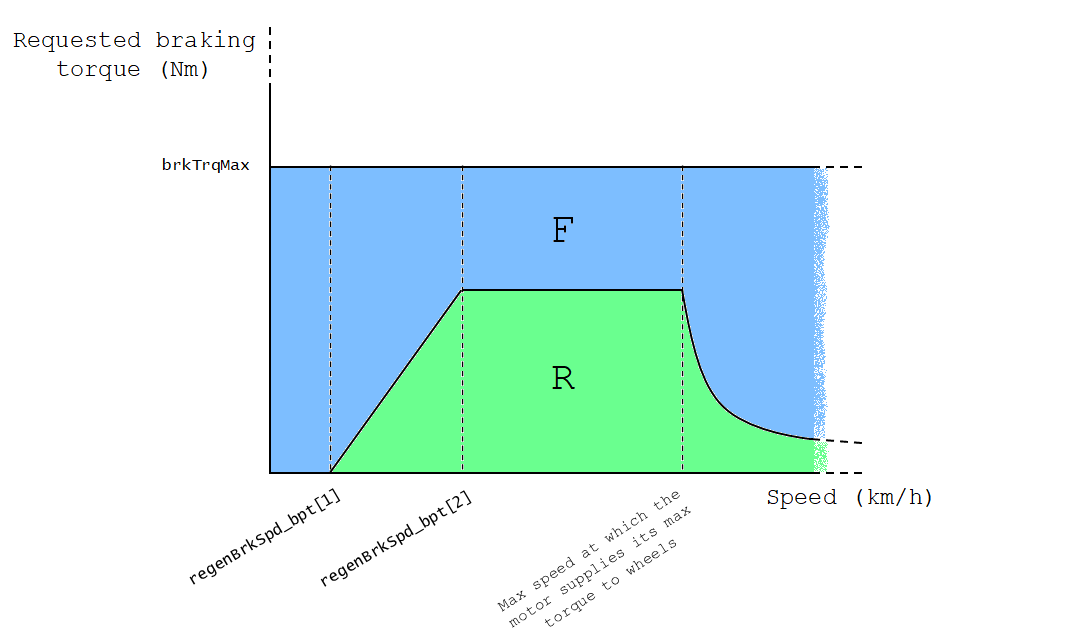
\includegraphics[width=\textwidth]{images/braking_distribution}
    \caption[Friction and regenerative braking torque distribution]{How the model distributes the requested braking torque between the regenerative (\texttt{R}) and friction (\texttt{F}) braking subsystems. Regenerative braking is activated when speed is above \texttt{RegenBrkSpd\_bpt[1]}. The maximum regenerative braking torque which can be supplied increases linearly with speed until a speed of \texttt{RegenBrkSpd\_bpt[2]} is reached. Above this speed, the regenerative brake is used to its full potential.}
    \label{fig:braking_distribution}
\end{figure}

The formula which models the maximum regenerative braking torque on each wheel given the speed $v$ of the vehicle is:
\begin{equation}
T_{regen} =
\begin{dcases}
    0 & \text{if } v \leq v_1\\
    \frac{v-v_1}{v_2-v_1} \cdot \frac{n_g T_{motor}(v)}{\eta_{regen}} & \text{if } v_1 < v \leq v_2\\
    \frac{n_g T_{motor}(v)}{\eta_{regen}} & \text{if } v > v_2\\
\end{dcases}
\end{equation}
where
\begin{itemize}
    \item $v_1$ (\texttt{RegBrkSpd\_bpt[1]}): cutoff speed above which the regenerative braking can be used [m/s]
    \item $v_2$ (\texttt{RegBrkSpd\_bpt[2]}): speed beyond which the regenerative brake can be used to its full potential [m/s]
    \item $n_g$ (\texttt{GR0*GRfinal}): overall gear ratio of the vehicle (see sec. \ref{sec:drivetrain})
    \item $T_{motor}(v)$ (previously written as $T_r(v)$ in sec. \ref{sec:motor}): maximum rotor torque at speed $v$ [N$\cdot$m]
    \item $\eta_{regen}$ (\texttt{regenEff}): efficiency factor for the regenerative braking
\end{itemize}
The negative torque $-T_{regen}/n_g$ is then used to control the motor (sec. \ref{sec:motor}), which will generate a negative current which recharges the battery pack.

\paragraph{Friction braking}
Friction braking is the conventional braking mechanism of all wheeled vehicles. A friction brake performs its function by pressing a brake pad against a rotating wheel. As a result, a friction force opposing the direction of the wheel is developed. In the process, the kinetic energy of the wheel is dissipated as heat.

Disc brakes (fig. \ref{fig:disc_brakes}) are the most commonly used form of friction brake for motor vehicles \cite{wiki:disc_brakes}. They are implemented in our EV model on all four wheels.

\begin{figure}[htb]
    \centering
    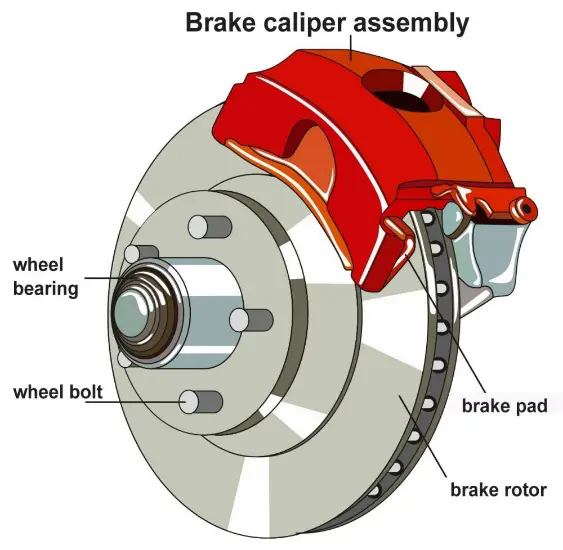
\includegraphics[width=0.45\textwidth]{images/disc_brakes}
    \caption[Disc brake]{Disc brake scheme. Taken from \cite{machinedesign_braking}}
    \label{fig:disc_brakes}
\end{figure}

The formula which models how much friction is generated on the wheel (measured as negative brake torque) is:
\begin{equation}
T_{disc} = \frac{\mu_{kinetic} P \pi d_{bore}^2 R_m N_{pads}}{4}
\label{eq:T_disc}
\end{equation}
where
\begin{itemize}
    \item $\mu_{kinetic}$ (\texttt{muKinetic}): coefficient of kinetic friction between disc pad and brake rotor
    \item $P$: total applied brake pressure [$\text{N}/\text{m}^2$]
    \item $d_{bore}$ (\texttt{discActBore}): brake actuator bore diameter [m]
    \item $R_m$ (\texttt{brakePadRadius}): mean radius of brake pad force application on the brake rotor [m]
    \item $N_{pads}$ (\texttt{numPads}): number of brake pads in the disc brake assembly
\end{itemize}
When the vehicle is still or the wheels are locked up (wheel skidding), the maximum friction braking torque on the wheel is still given by eq. \ref{eq:T_disc}, but $\mu_{static}$ (\texttt{muStatic}) is used in place of $\mu_{kinetic}$.

As anticipated, friction braking is used only when regenerative braking torque doesn't fulfil the braking torque request entirely: $T_{disc} = T_{braking} - T_{regen}$. The value $T_{disc}$ computed in this way is then used to compute the total pressure $P$ to be applied by the disc brakes to the wheels (sec. \ref{sec:wheels}), thanks to the inverse of eq. \ref{eq:T_disc}.



\subsection{Drivetrain}
\label{sec:drivetrain}
Drivetrain (also known as transmission, or driveline) is the set of rotating shafts and gears that distributes the mechanical power generated by the electric motor (sec. \ref{sec:motor}) to the wheels (sec. \ref{sec:wheels}).

While conventional internal combustion vehicles have a multi-gear gearbox with numerous ratios, nearly every electric car has a single-rate gearbox and no clutch, thus saving in cost, build complexity, weight and efficiency losses \cite{single_gear_ratio, ehsani_ev_book}. This is because electric motors have a much larger RPM range than the typical internal combustion engine (they often peak at about 20,000 RPM), they stay efficient across a very broad RPM range and produce a decent amount of torque at low RPM. EV designers pick a fixed gear ratio that provides a good compromise between acceleration and top speed \cite{single_gear_ratio}.

Gears are used across the drivetrain to reduce the angular velocity and increase torque before they are supplied to the wheels, while preserving power \cite{gear_trains}. A typical EV drivetrain is schematized in fig. \ref{fig:ev_drivetrain}. It consists of the gear between the motor and the driveshaft, the driveshaft, the differential (which houses the gear between the driveshaft and the drive axles), the two drive axles and the two drive wheels. Depending on the EV design, the drive wheels can be the rear or front ones (see sec. \ref{sec:wheels}); accordingly, the differential will be in the rear or front.

\begin{figure}[htb]
    \centering
    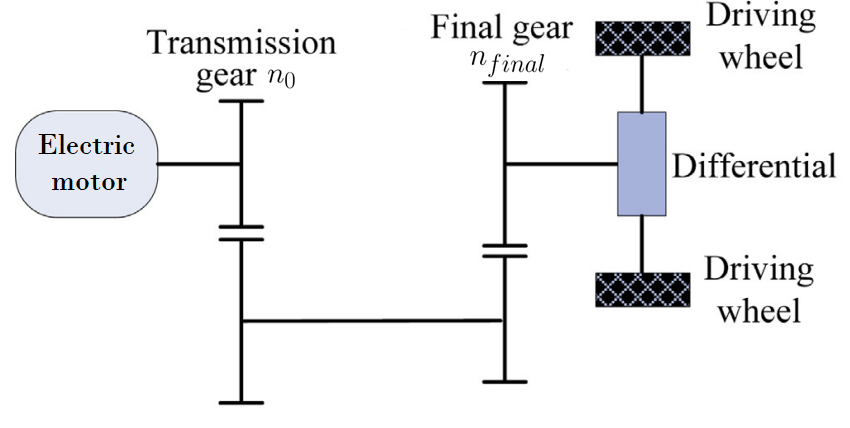
\includegraphics[width=0.7\textwidth]{images/ev_drivetrain}
    \caption[Drivetrain of an EV]{Schematic diagram of an EV drivetrain. Adapted from \cite{ev_drivetrain_schematic}}
    \label{fig:ev_drivetrain}
\end{figure}

The two gears have gear ratio $n_0$ and $n_{final}$, and efficiency of $\eta_0$ and $\eta_{final}$ (\texttt{GRfinal}) respectively; the driveshaft and drive axles have efficiency of $\eta_{ds}$ and $\eta_a$ respectively. It is convenient to express the overall gear ratio as
\begin{equation}
    n_g = n_0 \cdot n_{final}
\end{equation}
and the overall drivetrain efficiency as
\begin{equation}
    \eta_g = \eta_0 \cdot \eta_{ds} \cdot \eta_a \cdot \eta_{final}
\end{equation}

In the Simulink model, we simulate the components of the drivetrain with the following Simulink blocks:
\begin{itemize}
    \item First gear: Gearbox \cite{mathworks:gearbox}. Parameters: gear ratio $n_0$ (\texttt{GR0}), efficiency $\eta_0$ (\texttt{gearEff}).
    \item Driveshaft: Torsional Compliance \cite{mathworks:torsional_compliance}. Parameters: torsional stiffness $k_{ds}$ [N$\cdot$m/rad] (\texttt{driveshaft\_k}), damping $b_{ds}$ [N$\cdot$m$\cdot$s/rad] (\texttt{driveshaft\_b}), damping cutoff frequency $\omega_{ds}$ [rad/s] (\texttt{driveshaft\_wc}).
    \item Differential: Open Differential \cite{mathworks:differential}. Parameters: gear ratio $n_{final}$ (\texttt{GRfinal}), efficiency $\eta_{final}$ (\texttt{diffEff}).
    \item Drive axles: Torsional Compliance \cite{mathworks:torsional_compliance}. Parameters: torsional stiffness $k_a$ [N$\cdot$m/rad] (\texttt{axle\_k}), damping $b_a$ [N$\cdot$m$\cdot$s/rad] (\texttt{axle\_b}), damping cutoff frequency $\omega_a$ [rad/s] (\texttt{axle\_wc}).
\end{itemize}
Shaft efficiency can be computed from torsional stiffness, torsional damping and damping cutoff frequency\footnote{Note however that most EV manufacturers do not share such technical, low-level information about the vehicle components. For this reason, the user may want to stick with the default parameters taken from the model in \cite{racing_lounge}, which seem to work well in our experiments.}. The formula for computing it can be inferred from Simulink documentation \cite{mathworks:torsional_compliance}. 

If the vehicle is driven on a straight line, the torque at the differential is equally split between the left and right drive wheel. In this case, the torque that the drivetrain transmits from the motor to each drive wheel is computed as:
\begin{equation}
T_{wheel} = \frac{n_g \cdot \eta_{g} \cdot T_{motor}}{2}
\end{equation}
where
\begin{itemize}
    \item $n_g$: overall gear ratio
    \item $\eta_g$: total drivetrain efficiency
    \item $T_{motor}$: rotor torque [N$\cdot$m]
\end{itemize}



\subsection{Wheels}
\label{sec:wheels}
Wheels are modeled using the "Longitudinal wheel with disc brake" Simulink block \cite{mathworks:wheel}. The total longitudinal traction (or braking) force $F_x$ that the two drive wheels exert on the vehicle is given by Pacejka's Magic Formula \cite{magic_formula}:
\begin{equation}
F_x = F_z D \sin(C\arctan(B\kappa-E(B\kappa-\arctan(B\kappa))))
\end{equation}
where
\begin{itemize}
    \item $F_z$: vertical load on the tyre [N] (see sec. \ref{sec:body})
    \item $\kappa$: longitudinal wheel slip\footnote{Longitudinal wheel slip is defined as
    \[
    \kappa = -\frac{v-r_w\omega_w}{v}
    \]
    where $r_w$ and $\omega_w$ are respectively the wheel radius and wheel angular velocity, and $v$ is the longitudinal vehicle speed. When $\kappa=0$, the wheel is rolling without slipping; $\kappa>0$ means the wheel is slipping; $\kappa<0$ means the wheel is skidding.}
    \item $B, C, D, E$: stiffness, shape, peak and curvature factor
\end{itemize}
The four dimensionless coefficients are based on empirical data. We will assume that our EV model drives on dry tarmac, for which $B=10$, $C=1.9$, $D=1$, $E=0.97$ \cite{mathworks:wheel}. The block internally computes $\kappa$ knowing the wheel radius under load $r_w$ (\texttt{wheelRadius}), the vehicle speed $v$ and the torque that the drivetrain transfers to the wheel $T_{wheel}$ (sec. \ref{sec:drivetrain}).

This block also models the disc brake that operates on the wheel (sec. \ref{sec:braking}). When the disc brake is operated, $T_{wheel}$ is negative, therefore the computed $F_x$ is too (i.e. $F_x$ becomes a braking force).

Actually, tires are made of viscoelastic material, so they are subject to hysteresis energy loss, a phenomenon which results in rolling resistance \cite{rolling_resistance}. However, rolling resistance is not implemented in our model, as it would increase the complexity of the model and slow down the simulation. Nonetheless, one can take rolling resistance into account by using Pacejka's magic formula for rolling resistance (eq. 4.E70 of \cite{rolling_resistance}).
% https://www.youtube.com/watch?v=_S2lyaMgBQ8 see also first comment



\subsection{Vehicle body}
\label{sec:body}
The aerodynamic model of the vehicle body is implemented with the Vehicle Body 1DOF Longitudinal Simulink block \cite{mathworks:body}. It implements a one degree-of-freedom (1DOF) rigid vehicle body with constant mass undergoing longitudinal motion.

Assuming that the vehicle is driving on a flat road (angle of road grade $\gamma = 0$) with no wind, and that the two drive wheels are the front ones, this block internally solves the system of equations \ref{eq:free_body_system} associated to the vehicle's free body diagram (fig. \ref{fig:free_body_diagram}):
\begin{equation}
\begin{dcases}
    F_x = m\Ddot{x}\\
    F_x = F_{xF} + F_{xR} - F_{d,x}\\
    F_{d,x} = \frac{1}{2T_{air}R_{air}} C_d A_f P_{air} \dot{x}^2\\
    F_{zF} = \frac{bmg - h (F_{xF} + F_{xR})}{2(a+b)}\\
    F_{zR} = \frac{amg + h (F_{xF} + F_{xR})}{2(a+b)}\\
\end{dcases}
\label{eq:free_body_system}
\end{equation}

where
\begin{itemize}
    \item $F_x$: effective longitudinal force [N]
    \item $F_{xF}, F_{xR}$: total longitudinal force exerted by the two front (F) and rear (R) wheels [N]
    \item $F_{d,x}$: longitudinal aerodynamic drag force [N]
    \item $F_{zF}, F_{zR}$: normal load force on each front (F) and rear (R) wheel [N]
    \item $a$ (\texttt{a}): horizontal distance from vehicle's center of gravity (CG) to rear axle [m]
    \item $b$ (\texttt{b}): horizontal distance from vehicle's CG to front axle [m]
    \item $h$ (\texttt{h}): vehicle's CG height above axles [m]
    \item $m$ (\texttt{vehicleMass}): vehicle loaded mass [kg]
    \item $\Ddot{x}$: vehicle longitudinal acceleration [m/s\textsuperscript{2}]
    \item $A_f$ (\texttt{frontalArea}): vehicle's frontal area [m\textsuperscript{2}]
    \item $C_d$ (\texttt{dragCoeff}): frontal air drag coefficient
    \item $T_{air}, P_{air}, R_{air}$: air temperature [K], pressure [Pa] and specific gas constant [J$\cdot$kg\textsuperscript{-1}$\cdot$K\textsuperscript{-1}]
\end{itemize}

\begin{figure}[hbt!]
\centering
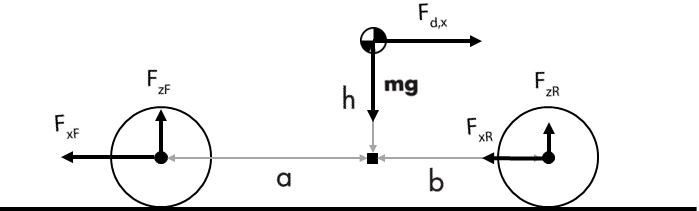
\includegraphics[width=0.8\textwidth]{images/free_body_diagram}
\caption[Free body diagram of a vehicle]{Free body diagram of the vehicle model. Adapted from \cite{mathworks:body}}
\label{fig:free_body_diagram}
\end{figure}

Given $F_{xF}$ and $F_{xR}$ (sec. \ref{sec:wheels}), the block outputs the vehicle speed $v$ and the normal load forces $F_{zF}$ and $F_{zR}$.



\subsection{Battery pack}
\label{sec:battery_pack}
The EV's battery pack is the most critical component of the model, since our aim is to predict its SOH. As discussed in sec. \ref{sec:li-ion}, an EV battery pack is actually a set of battery cells connected together in series and parallel; however, modeling an EV battery pack at the cell level would greatly increase the complexity of the simulation, and would be very hard to parametrize in a realistic way without extensive knowledge of the specific topology of the pack, its positioning inside the car and the specific features of the BMS in use. Therefore, we model our battery pack as if it consisted of only one high-voltage cell. To do so, our model uses the Generic Battery Model (GBM) block from the Simscape electrical Simulink library \cite{mathworks:battery}.
This block implements a generic dynamic equivalent circuit model (ECM) of a rechargeable battery, summarized in fig. \ref{fig:battery_ECM}.

\begin{figure}[htb]
    \centering
    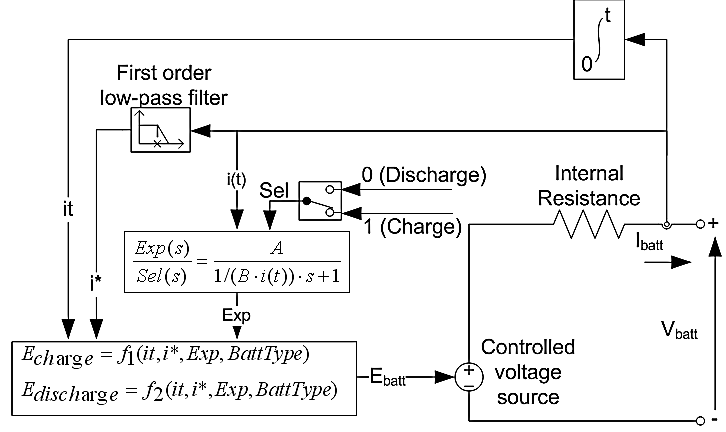
\includegraphics[width=0.8\textwidth]{images/battery_ECM.png}
    \caption[GBM internal ECM model]{Internal ECM model of the Generic Battery Model Simulink block. Taken from \cite{mathworks:battery}}
    \label{fig:battery_ECM}
\end{figure}

The GBM block interacts with the rest of the EV model as described in sec. \ref{sec:motor}: the motor reads the terminal voltage of the battery pack $V_{batt}$ and requests a current $I_{batt}$ based on the power demand $P_{batt}$. Then, a controlled current source imposes a current $I_{batt}$ to the battery pack, causing the terminal voltage to change accordingly to the charge/discharge characteristics specified for the battery pack (see "Discharge characteristics" paragraph). Moreover, the battery pack thermally interacts with the environment by reading the external temperature $T_a$, which can be set by the user. The equations which govern the electrical and thermal dynamics of the battery can be found in \cite{mathworks:battery}.

The GBM block parameters must be set according to those characterizing the battery pack of the specific EV we want to model. The parameters required to initialize the block are briefly discussed in the following paragraphs.

\subsubsection{Discharge characteristics}
\label{sec:discharge_characteristics}
In fig. \ref{fig:discharge_curve} a typical discharge curve of a battery cell is plotted. Three distinct sections can be observed:
\begin{enumerate}
    \item \textit{Exponential zone}: exponential voltage drop from a fully charged state $(V_{full},0)$ to a point $(V_{exp},Q_{exp})$;
    \item \textit{Nominal zone}: characterized by an almost constant voltage; from $(V_{exp},Q_{exp})$ to $(V_{nom},Q_{nom})$;
    \item \textit{Total discharge zone}: an extremely rapid voltage drop from $(V_{nom},Q_{nom})$ to $(V_{empty},Q_{full})$.
\end{enumerate}

\begin{figure}[htb]
    \centering
    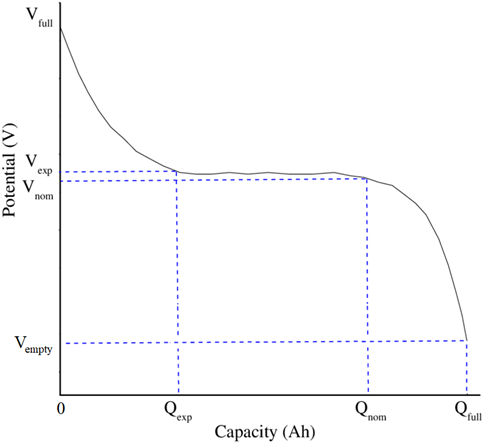
\includegraphics[width=0.7\textwidth]{images/discharge_curve.png}
    \caption[Discharge curve of a battery]{Typical discharge curve of a battery (at a certain C-rate, temperature, SOH), function of the discharged capacity $Q$. NB: the curve is not in scale, as the nominal zone is typically much wider compared to the exponential and total discharge zones.}
    \label{fig:discharge_curve}
\end{figure}

The discharge characteristics depend on a set of nominal conditions of operation defined by a nominal ambient temperature $T_{nom}$ (\texttt{Tnom1}) and a nominal discharge current $I_{nom}$ (\texttt{nomDischCurr}). To internally model the discharge curve in such operating conditions, the block requires the following parameters to be set:
\begin{itemize}
\item $Q_{rated}$ (\texttt{ratedCap}): rated capacity, i.e. the minimum effective capacity of the battery [Ah]
\item $R_{int}$ (\texttt{intRes}): internal resistance when the battery is fresh [$\Omega$]
\item $V_{full}$ (\texttt{fullychargV}): voltage at which the battery is fully charged [V]
\item $V_{exp}$ (\texttt{expV}): voltage at the end of the exponential zone [V]
\item $Q_{exp}$ (\texttt{expVCap}): discharged capacity at $V_{exp}$ [Ah]
\item $V_{nom}$ (\texttt{nomV}): voltage at the end of the nominal zone [V]
\item $Q_{nom}$ (\texttt{nomVCap}): discharged capacity at $V_{nom}$ [Ah]
\item $V_{empty}$ (\texttt{cutoffV}): voltage at which the battery is fully discharged [V]
\item $Q_{full}$ (\texttt{maxCap}): maximum theoretical capacity [Ah]
\end{itemize}

The user must also provide the SOC (\%) of the battery at the beginning of the simulation (\texttt{initSOC}). Finally, self-discharge is modeled by adding a large resistor of 2000 $\Omega$ in parallel with the battery terminals.

\subsubsection{Thermal model}
\label{sec:thermal_model}
The following parameters describe the discharge characteristics at a second operating condition (different from the nominal one), characterized by an external temperature $T_{nom,2}$ (\texttt{Tnom2}):
\begin{itemize}
\item $Q_{full,2}$ (\texttt{maxCap\_Tnom2}): maximum theoretical capacity [Ah]
\item $V_{full,2}$ (\texttt{initDischV\_Tnom2}): voltage at which the battery is fully charged [V]
\item $V_{90\%}$ (\texttt{V90maxCap\_Tnom2}): voltage when 90\% of $Q_{full,2}$ has been discharged [V]
\item $V_{exp,2}$ (\texttt{expV\_Tnom2}): voltage at the end of the exponential zone [V]
\item $Q_{exp,2}$ (\texttt{expVCap\_Tnom2}): discharged capacity at $V_{exp,2}$ [Ah]
\end{itemize}

Moreover, battery-to-ambient thermal interaction is described by two parameters: thermal resistance (\texttt{thRes}) and thermal time constant (\texttt{thTimeConst}). The user must also provide the internal temperature [°C] of the battery at the beginning of the simulation (\texttt{initBattTemp}), and the external temperature $T_a$ [°C], which can either be a constant or a time series of temperature measurements.

\subsubsection{Aging model}
\label{sec:aging_model}
Other than current and internal temperature, discharge characteristics are also affected by battery pack's SOH. The GBM block features a simple aging model of the battery, which is parametrized with the following parameters:
\begin{itemize}
    \item $Q_{EOL}$: maximum theoretical capacity at end of life [Ah]; usually for EV applications, battery pack's EOL is set at 80\% $Q_{full}$ (i.e. $0.8\times\text{\texttt{maxCap}}$) \cite{cap_eol}.
    \item $R_{EOL}$: internal resistance at end of life [$\Omega$]; set to $2\times\text{\texttt{intRes}}$ by default \cite{r_eol}.
    \item $I_c, I_{c,max}$ (\texttt{Ic, Icmax}): nominal and maximum charge current [A]
    \item $I_d, I_{d,max}$ (\texttt{Id, Idmax}): nominal and maximum discharge current [A]
    \item \texttt{cycLife\_100DOD\_Ic\_Id\_Ta1}: EFC at 100\% DOD, at $I_c$ and $I_d$, to reach EOL
    \item \texttt{cycLife\_25DOD\_Ic\_Id\_Ta1}: EFC at 25\% DOD, at $I_c$ and $I_d$, to reach EOL
    \item \texttt{cycLife\_100DOD\_Ic\_Idmax\_Ta1}: EFC at 100\% DOD, at $I_c$ and $I_{d,max}$, to reach EOL
    \item \texttt{cycLife\_100DOD\_Icmax\_Id\_Ta1}: EFC at 100\% DOD, at $I_{c,max}$ and $I_d$, to reach EOL
    \item $T_{amb,2}$ (\texttt{Ta2}): a second ambient temperature at which the aging model is parametrized [°C]
    \item \texttt{cycLife\_100DOD\_Ic\_Id\_Ta2}: EFC at 100\% DOD, at $I_c$ and $I_d$ and temperature $T_{amb,2}$, to reach EOL
\end{itemize}
The user must also specify the battery age (as number of EFC) which characterizes the battery pack throughout the simulation (\texttt{initBattAge}).

The mathematical relationship between the battery age expressed in number of EFC and the percentage of fresh maximum capacity (which is our reference definition of SOH, eq. \ref{eq:soh}) is not linear in general \cite{efc_vs_soh}. However, a simple simulation of a battery characterization test may be performed to unambiguously associate an EFC level to the correspondent SOH value (sec. \ref{sec:efc2soh}).



\subsection{Known limitations}
\label{sec:known_limitations}
Our proposed EV model suffers from several limitations, mainly due to its low-complexity design. Known limitations are:
\begin{itemize}
    \item Energy losses due to auxiliary devices (such as air-conditioner, power steering, car lights and so on), which are usually powered by a 12V auxiliary battery \cite{auxiliary_battery}, are not modeled.
    \item Rolling resistance is not modeled, as explained in sec. \ref{sec:wheels}.
    \item It is often difficult to retrieve technical specifications of a specific EV model from the Internet, as this information is not always publicly shared by EV manufacturers. Required specifications which could not be found have been estimated indirectly by exploiting real EV field data or otherwise made up by choosing plausible values.
    \item Many EVs can operate in different driving modes, with the aim of adapting the energy consumption to a desired driving profile, ultimately optimizing the vehicle's driving range \cite{vw_driving_modes}. Due to the huge variety of driving modes implemented by different EV manufacturers, the model is designed with a default driving mode.
    \item A fair validation of the Simulink EV model by means of monitoring data acquired from real EVs is impossible, because an EV's BMS monitors only a fraction of the many different variables and factors which characterize driving. For instance: road type, slope, road curves, wind direction and speed are usually not recorded. For this reason, our model is designed to mimic the dynamics of a car moving in the forward direction on a flat dry tarmac road.
    \item The ECM model which characterizes Simulink generic battery block (sec. \ref{sec:battery_pack}) has several limitations and assumptions in its design, as stated in its documentation \cite{mathworks:battery}. For instance:
    \begin{itemize}
        \item internal resistance is assumed to be constant during charging and discharging and does not vary with the amplitude of the current;
        \item the capacity of the battery does not change with the amplitude of the current (there is no Peukert effect);
        \item the battery has no memory effect.
    \end{itemize}
    \item Simulink generic battery block implements a very low complexity thermal model, which cannot precisely capture heat transfer phenomena at the cell and module level and between the heat-producing components of the car (e.g. the motor) and the battery itself. Moreover, the thermal behaviour of the block seems to be independent of the SOH of the battery (as opposed to real batteries, as discussed in sec. \ref{sec:li-ion}). % However, this is not a big deal, because temperature doesn't affect SOH so much: https://onlinelibrary.wiley.com/doi/epdf/10.1002/er.6005
    \item The user cannot specify battery's SOH directly, but rather the battery age expressed in number of EFC; this limitation is overcome by mapping EFC levels to SOH values (see sec. \ref{sec:efc2soh}).
\end{itemize}





\section{EV model parametrization}
\label{sec:model_parametrization}
In order to generate a synthetic dataset of monitoring data, the EV Simulink model must be parametrized according to the technical specifications of a specific EV model. In this thesis, we focus on two EV models by Volkswagen: the e-up! (18.7 kWh) and the e-Golf (35.8 kWh). This choice is due to the availability of real driving session monitoring data for these two models (sec. \ref{sec:aviloo_ds}), acquired from a private EV fleet management company (sec. \ref{sec:aviloo}).

The required technical specifications for the VW e-up! and VW e-Golf are reported in table \ref{tab:eup_egolf_specs}. As mentioned in sec. \ref{sec:known_limitations}, retrieving the actual technical specifications for an EV model is not an easy task in general. For this reason, whenever any specification was not directly found on the Internet or in the literature it has been either:
\begin{itemize}
\item estimated with a parameter estimation procedure (see sec. \ref{sec:parameter_estimation}); marked with "\textbf{est}" in table \ref{tab:eup_egolf_specs}
\item computed indirectly from pertaining sources, assumed from sources pertaining to similar models, or otherwise left as Simulink's default value; marked with "\textbf{*}" in table \ref{tab:eup_egolf_specs}
\end{itemize}





\newgeometry{left=2.05cm,right=2.05cm,footskip=20mm}

\begin{table}[H]
\scriptsize
\centering
\captionsetup{size=small}
\caption[Technical specifications for the VW e-up! and the VW e-Golf]{Technical specifications for the VW e-up! (18.7 kWh) and the VW e-Golf (35.8 kWh). Parameters marked with 'est' are estimated through parameter estimation (sec. \ref{sec:parameter_estimation}), and those marked with '*' are computed indirectly from pertaining sources or left as default.}
\label{tab:eup_egolf_specs}
\begin{tabular}[t]{cllccccc}
\toprule
& \breakcellleft{Parameter\\name} & \breakcellleft{Workspace\\variable} & e-up! & e-Golf & Unit & \breakcell{Source\\(e-up!)} & \breakcell{Source\\(e-Golf)} \\
\midrule
\multirow{12}{*}{\STAB{\rotatebox[origin=c]{90}{Motor}}}
& Rotor speed breakpoints & \texttt{motorSpdRPM} & (see source) & (see source) & RPM & \cite{motorSpdRPM-eup} & \cite{motorSpdRPM-egolf}
\\[0.15cm]
& \breakcellleft{Max. motor torque at\\rotor speed breakpoints} & \texttt{motorMaxTrq} & (see source) & (see source) & N$\cdot$m & \cite{motorSpdRPM-eup} & \cite{motorSpdRPM-egolf}
\\[0.28cm]
& Motor efficiency & \texttt{motorEff} & 0.95 & 0.95 & -- & \cite{motorEff1,motorEff2},* & \cite{motorEff1,motorEff2},*
\\[0.15cm]
& \breakcellleft{Rotor speed at which\\motor eff. is measured} & \texttt{motorEffSpd} & 6500 & 6500 & RPM & \cite{motorSpdRPM-eup,motorEff2},* & \cite{motorSpdRPM-egolf,motorEff2},*
\\[0.28cm]
& \breakcellleft{Rotor torque at which\\motor eff. is measured} & \texttt{motorEffTrq} & 89 & 146 & N$\cdot$m & \cite{motorSpdRPM-eup,motorEff2},* & \cite{motorSpdRPM-egolf,motorEff2},*
\\[0.28cm]
& Iron losses & \texttt{motorPIron} & 0 & 0 & W & * & *
\\[0.15cm]
& Fixed losses & \texttt{motorPBase} & 0 & 0 & W & * & *
\\[0.15cm]
\midrule
\multirow{13}{*}{\STAB{\rotatebox[origin=c]{90}{Braking system}}}
& \breakcellleft{Max. total braking\\torque} & \texttt{brqTrqMax} & 2000 & 2000 & N$\cdot$m & \cite{brkTrqMax},* & \cite{brkTrqMax},*
\\[0.28cm]
& \breakcellleft{Regen. braking cutoff\\speeds} & \texttt{RegenBrkSpd\_bpt} & [18, 32.4] & [18, 32.4] & km/h & \cite{racing_lounge},* & \cite{racing_lounge},*
\\[0.28cm]
& Regen. efficiency factor & \texttt{regenEff} & 0.75 & 0.75 & -- & \cite{racing_lounge},* & \cite{racing_lounge},*
\\[0.15cm]
& Kinetic friction coeff. & \texttt{muKinetic} & 0.35 & 0.35 & -- & \cite{racing_lounge},* & \cite{racing_lounge},*
\\[0.15cm]
& Static friction coeff. & \texttt{muKinetic} & 0.9 & 0.9 & -- & \cite{racing_lounge},* & \cite{racing_lounge},*
\\[0.15cm]
& \breakcellleft{Brake actuator bore\\diameter} & \texttt{discActBore} & 0.05 & 0.05 & m & \cite{racing_lounge},* & \cite{racing_lounge},*
\\[0.28cm]
& Brake pad radius & \texttt{brakePadRadius} & 0.15 & 0.15 & m & \cite{racing_lounge},* & \cite{racing_lounge},*
\\[0.15cm]
& N. of brake pads & \texttt{numPads} & 2 & 2 & -- & \cite{racing_lounge},* & \cite{racing_lounge},*
\\[0.15cm]
\midrule
\multirow{16}{*}{\STAB{\rotatebox[origin=c]{90}{Drivetrain}}}
& First gear ratio & \texttt{GR0} & 1.576 & 2.7 & -- & \cite{eup_tech_specs1} & \cite{egolf_tech_specs1}
\\[0.15cm]
& First gear efficiency & \texttt{gearEff} & 0.95 & 0.95 & -- & \cite{gearEff},* & \cite{gearEff},*
\\[0.15cm]
& Driveshaft tors. stiffness & \texttt{driveshaft\_k} & 2500 & 2500 & N$\cdot$m/rad & \cite{racing_lounge},* & \cite{racing_lounge},*
\\[0.15cm]
& Driveshaft tors. damping & \texttt{driveshaft\_b} & 10 & 10 & N$\cdot$m$\cdot$s/rad & \cite{racing_lounge},* & \cite{racing_lounge},*
\\[0.15cm]
& \breakcellleft{Driveshaft damping\\cutoff frequency} & \texttt{driveshaft\_wc} & 500 & 500 & rad/s & \cite{racing_lounge},* & \cite{racing_lounge},*
\\[0.28cm]
& Final gear ratio & \texttt{GRfinal} & 5.176 & 3.61 & -- & \cite{eup_tech_specs1} & \cite{egolf_tech_specs1}
\\[0.15cm]
& Differential efficiency & \texttt{diffEff} & 0.95 & 0.95 & -- & \cite{gearEff},* & \cite{gearEff},*
\\[0.15cm]
& Axle tors. stiffness & \texttt{axle\_k} & 5000 & 5000 & N$\cdot$m/rad & \cite{racing_lounge},* & \cite{racing_lounge},*
\\[0.15cm]
& Axle tors. damping & \texttt{axle\_b} & 10 & 10 & N$\cdot$m$\cdot$s/rad & \cite{racing_lounge},* & \cite{racing_lounge},*
\\[0.15cm]
& \breakcellleft{Axle damping\\cutoff frequency} & \texttt{axle\_wc} & 400 & 400 & rad/s & \cite{racing_lounge},* & \cite{racing_lounge},*
\\[0.28cm]
\midrule
\multirow{10}{*}{\STAB{\rotatebox[origin=c]{90}{Body and wheels}}}
& Wheel radius & \texttt{wheelRadius} & 0.293 & 0.316 & m & \cite{eup_tech_specs1,wheelRadius_calc} & \cite{egolf_tech_specs1,wheelRadius_calc}
\\[0.15cm]
& CG to front axle & \texttt{a} & 1.04 & 1.21 & m & \cite{eup_tech_specs3,eup_tech_specs4,CG_calc} & \cite{egolf_tech_specs1,egolf_tech_specs2,CG_calc}
\\[0.15cm]
& CG to rear axle & \texttt{b} & 1.38 & 1.42 & m & \cite{eup_tech_specs3,eup_tech_specs4,CG_calc} & \cite{egolf_tech_specs1,egolf_tech_specs2,CG_calc}
\\[0.15cm]
& CG height above axles & \texttt{h} & 0.35 & 0.35 & m & \cite{racing_lounge},* & \cite{racing_lounge},*
\\[0.15cm]
& Vehicle mass & \texttt{vehicleMass} & 1375 & 1690 & kg & \cite{eup_tech_specs2} & \cite{egolf_tech_specs1}
\\[0.15cm]
& Frontal area & \texttt{frontalArea} & 2.07 & 2.21 & m\textsuperscript{2} & \cite{eup_tech_specs3},* & \cite{egolf_tech_specs3},*
\\[0.15cm]
& Air drag coefficient & \texttt{dragCoeff} & 0.32 & 0.27 & -- & \cite{eup_tech_specs2} & \cite{egolf_tech_specs1}
\\[0.15cm]
\midrule
\multicolumn{8}{r}{continued on next page}\\
%\bottomrule
\end{tabular}
\end{table}

\begin{table}[H]
\scriptsize
\centering
\captionsetup{justification=centering,size=small}
\caption*{\textbf{Table \ref{tab:eup_egolf_specs}} (continued)}
\begin{tabular}[t]{cllccccc}
\multicolumn{8}{l}{continued from previous page}\\[0.15cm]
\toprule
& \breakcellleft{Parameter\\name} & \breakcellleft{Workspace\\variable} & e-up! & e-Golf & Unit & \breakcell{Source\\(e-up!)} & \breakcell{Source\\(e-Golf)} \\
\midrule
\multirow{17}{*}{\STAB{\rotatebox[origin=c]{90}{Battery pack - discharge}}}
& Nom. amb. temperature & \texttt{Tnom1} & 20 & 20 & °C & \cite{mathworks:battery} & \cite{mathworks:battery}
\\[0.15cm]
& Nom. disch. current & \texttt{nomDischCurr} & 24.8 & 54.2 & A & est & est
\\[0.15cm]
& Rated capacity & \texttt{ratedCap} & 50.3 & 116.1 & Ah & \cite{eup_tech_specs2}, est & \cite{egolf_tech_specs1}, est
\\[0.15cm]
& Internal resistance & \texttt{intRes} & 0.08 & 0.075 & $\Omega$ & \cite{intRes}, est & \cite{intRes}, est
\\[0.15cm]
& Voltage at 100\% SOC & \texttt{fullychargV} & 429.9 & 386.6 & V & \cite{eup_tech_specs5}, est & \cite{intRes}, est
\\[0.15cm]
& \breakcellleft{Voltage at the end of\\the exp. zone ($V_{exp}$)} & \texttt{expV} & 407.6 & 351.9 & V & est & est
\\[0.28cm]
& Capacity disch. at $V_{exp}$ & \texttt{expVCap} & 5.0 & 10.6 & Ah & est & est
\\[0.15cm]
& \breakcellleft{Voltage at the end of\\the nom. zone ($V_{nom}$)} & \texttt{nomV} & 345.6 & 304.3 & V & \cite{eup_tech_specs2}, est & \cite{egolf_tech_specs1}, est
\\[0.15cm]
& Capacity disch. at $V_{nom}$ & \texttt{expVCap} & 44.0 & 95.8 & Ah & est & est
\\[0.15cm]
& Voltage at 0\% SOC & \texttt{cutoffV} & 297.2 & 288.7 & V & \cite{eup_tech_specs5}, est & \cite{intRes}, est
\\[0.15cm]
& Max. theor. capacity & \texttt{maxCap} & 49.9 & 107.7 & Ah & est & est
\\[0.15cm]
\cmidrule{2-8}
\multirow{17}{*}{\STAB{\rotatebox[origin=c]{90}{Battery pack - thermal}}}
& \breakcellleft{2nd nom. amb.\\temperature ($T_{nom,2}$)} & \texttt{Tnom2} & -30 & -30 & °C & \cite{mathworks:battery} & \cite{mathworks:battery}
\\[0.28cm]
& \breakcellleft{Max. theor. capacity\\at $T_{nom,2}$} & \texttt{maxCap\_Tnom2} & 38.3 & 87.9 & Ah & est & est
\\[0.28cm]
& \breakcellleft{Voltage at 100\% SOC\\at $T_{nom,2}$} & \texttt{initDischV\_Tnom2} & 397.2 & 350.2 & V & est & est
\\[0.28cm]
& \breakcellleft{Voltage when 90\% disch.\\cap., at $T_{nom,2}$} & \texttt{V90maxCap\_Tnom2} & 304.5 & 289.8 & V & est & est
\\[0.28cm]
& \breakcellleft{Voltage at the end of\\the exp. zone, at\\$T_{nom,2}$ ($V_{exp,2}$)} & \texttt{expV\_Tnom2} & 392.2 & 326.9 & V & est & est
\\[0.45cm]
& \breakcellleft{Cap. discharged at\\$V_{exp,2}$, at $T_{nom,2}$} & \texttt{expVCap\_Tnom2} & 2.0 & 9.9 & Ah & est & est
\\[0.28cm]
& Thermal resistance & \texttt{thRes} & 0.065 & 0.013 & °C/W & est & est
\\[0.15cm]
& Thermal time constant & \texttt{thTimeConst} & 30000 & 27000 & s & est & est
\\[0.15cm]
\cmidrule{2-8}
\multirow{20}{*}{\STAB{\rotatebox[origin=c]{90}{Battery pack - aging}}}
& Nom. charge current & \texttt{Ic} & 7.5 & 7.5 & A & * & *
\\[0.15cm]
& Max. charge current & \texttt{Icmax} & 9.58 & 9.58 & A & * & *
\\[0.15cm]
& Nom. discharge current & \texttt{Id} & 17.83 & 17.83 & A & * & *
\\[0.15cm]
& Max. discharge current & \texttt{Idmax} & 75.93 & 75.93 & A & * & *
\\[0.15cm]
& \breakcellleft{EFC @ 100\% DOD,\\$I_c$, $I_d$ to EOL} & \texttt{cycLife\_100DOD\_Ic\_Id\_Ta1} & 3000 & 3000 & -- & \cite{battery_research},* & \cite{battery_research},*
\\[0.28cm]
& \breakcellleft{EFC @ 25\% DOD,\\$I_c$, $I_d$ to EOL} & \texttt{cycLife\_25DOD\_Ic\_Id\_Ta1} & 20000 & 20000 & -- & * & *
\\[0.28cm]
& \breakcellleft{EFC @ 100\% DOD,\\$I_c$, $I_{d,max}$ to EOL} & \texttt{cycLife\_100DOD\_Ic\_Idmax\_Ta1} & 2000 & 2000 & -- & \cite{battery_research},* & \cite{battery_research},*
\\[0.28cm]
& \breakcellleft{EFC @ 100\% DOD,\\$I_{c,max}$, $I_d$ to EOL} & \texttt{cycLife\_25DOD\_Icmax\_Id\_Ta1} & 2500 & 2500 & -- & \cite{battery_research},* & \cite{battery_research},*
\\[0.28cm]
& \breakcellleft{2nd amb. temperature\\($T_{amb,2}$)} & \texttt{Ta2} & 45 & 45 & °C & \cite{mathworks:battery} & \cite{mathworks:battery}
\\[0.28cm]
& \breakcellleft{EFC @ 100\% DOD,\\$I_c$, $I_d$, $T_{amb,2}$ to EOL} & \texttt{cycLife\_100DOD\_Ic\_Id\_Ta2} & 2500 & 2500 & -- & * & *
\\[0.28cm]
\bottomrule
\end{tabular}
\end{table}

\restoregeometry





\subsection{Parameter estimation}
\label{sec:parameter_estimation}
Most parameters specific to the battery pack have been estimated with Simulink Parameter Estimator app \cite{mathworks:parameter_estimator}. Parameter estimation can be formulated as a constrained or unconstrained optimization problem (sec. \ref{sec:opt_prob}).

The parameters estimated with this procedure are those marked with "est" in table \ref{tab:eup_egolf_specs}. We set up a parameter estimation experiment by picking a real driving session from each of the two acquired real datasets to use as experimental input and output data. The battery pack current signals from the two driving sessions have been extracted and set as the input signals for the simulation. We have chosen two battery test driving sessions, as they produce signals spanning from a full charge to an almost full discharge of the battery pack: these wide operating conditions ensure that the found parameters are well-fitted for almost any section of the discharge curve of the battery pack. The initial SOC, initial battery temperature and battery SOH of the simulated battery pack are set accordingly to the selected driving session. The battery pack voltages have been chosen as the measured output signals; parameters have been tuned so that the simulated voltage signal matches the experimental one as much as possible (i.e. the SSE over the measured signal time base\footnote{The measured signal time base consists of all the timestamps for which the measured signal is specified, whereas the simulated signal time base consists of all the timestamps for which the model is simulated. The two time bases are different in general. By default, Simulink Parameter Estimator computes the cost function only in the timestamps of the measured signal time base. Our Simulink model uses a variable-step discrete solver, which adjusts the simulation step size during the simulation by reducing it to increase accuracy when model states are changing rapidly and increasing it to avoid taking unnecessary steps when model states are changing slowly; therefore, it can always simulate the model in the specific timestamps of the measured signal time base, if informed to do so.} is minimized). Nelder-Mead method (sec. \ref{sec:nelder_mead}) has been chosen to solve the optimization problem.

The value for each parameter to be estimated has been initialized randomly in a plausible value interval for the battery pack under consideration. The chosen value intervals are compatible with the electrical parameters reported in tab. \ref{tab:eup_egolf_specs}, and are reported in tab. \ref{tab:par_est_search_intervals} for each parameter to be estimated. Nelder-Mead optimization method solves the parameter estimation problem in an unconstrained way.

\begin{table}[hbt!]
\centering
\begin{tabular}[t]{lccc}
\toprule
Parameter & \breakcell{Search interval\\(e-up!)} & \breakcell{Search interval\\(e-Golf)} & Unit\\
\midrule
\texttt{nomV} & $[330,\;390]$ & $[300,\;360]$ & V\\[0.1cm]
\texttt{ratedCap} & $[45,\;55]$ & $[105,\;115]$ & Ah\\[0.1cm]
\texttt{maxCap} & $[50,\;60]$ & $[108,\;125]$ & Ah\\[0.1cm]
\texttt{cutoffV} & $[270,\;310]$ & $[250,\;280]$ & V\\[0.1cm]
\texttt{fullychargV} & $[405,\;435]$ & $[345,\;375]$ & V\\[0.1cm]
\texttt{nomDischCurr} & $[25,\;30]$ & $[50,\;60]$ & A\\[0.1cm]
\texttt{intRes} & $[0.06,\;0.1]$ & $[0.06,\;0.1]$ & $\Omega$\\[0.1cm]
\texttt{nomVCap} & $[35,\;48]$ & $[75,\;105]$ & Ah\\[0.1cm]
\texttt{expV} & $[390,\;420]$ & $[325,\;360]$ & V\\[0.1cm]
\texttt{expVCap} & $[0,\;10]$ & $[0,\;20]$ & Ah\\[0.1cm]
\texttt{maxCap\_Tnom2} & $[30,\;45]$ & $[66,\;100]$ & Ah\\[0.1cm]
\texttt{initDischV\_Tnom2} & $[390,\;415]$ & $[325,\;355]$ & V\\[0.1cm]
\texttt{V90maxCap\_Tnom2} & $[290,\;330]$ & $[270,\;300]$ & Ah\\[0.15cm]
\texttt{expV\_Tnom2} & $[375,\;405]$ & $[305,\;345]$ & V\\[0.1cm]
\texttt{expVCap\_Tnom2} & $[0,\;10]$ & $[0,\;20]$ & Ah\\
\bottomrule
\end{tabular}
\caption[Initialization intervals for the parameter estimator]{Initialization intervals for each parameter to be tuned.}
\label{tab:par_est_search_intervals}
\end{table}

Fig. \ref{fig:par_est_comparison_V} and \ref{fig:par_est_comparison_SOC} show a comparison of the simulated voltage and SOC signals versus the experimental (real) ones. In both cases, the simulated signals tend to mimic the experimental ones with a very low error (as high as 10 V for the voltage signals).

\begin{figure}[htbp!]
\centering
\begin{subfigure}{\textwidth}
    \centering
    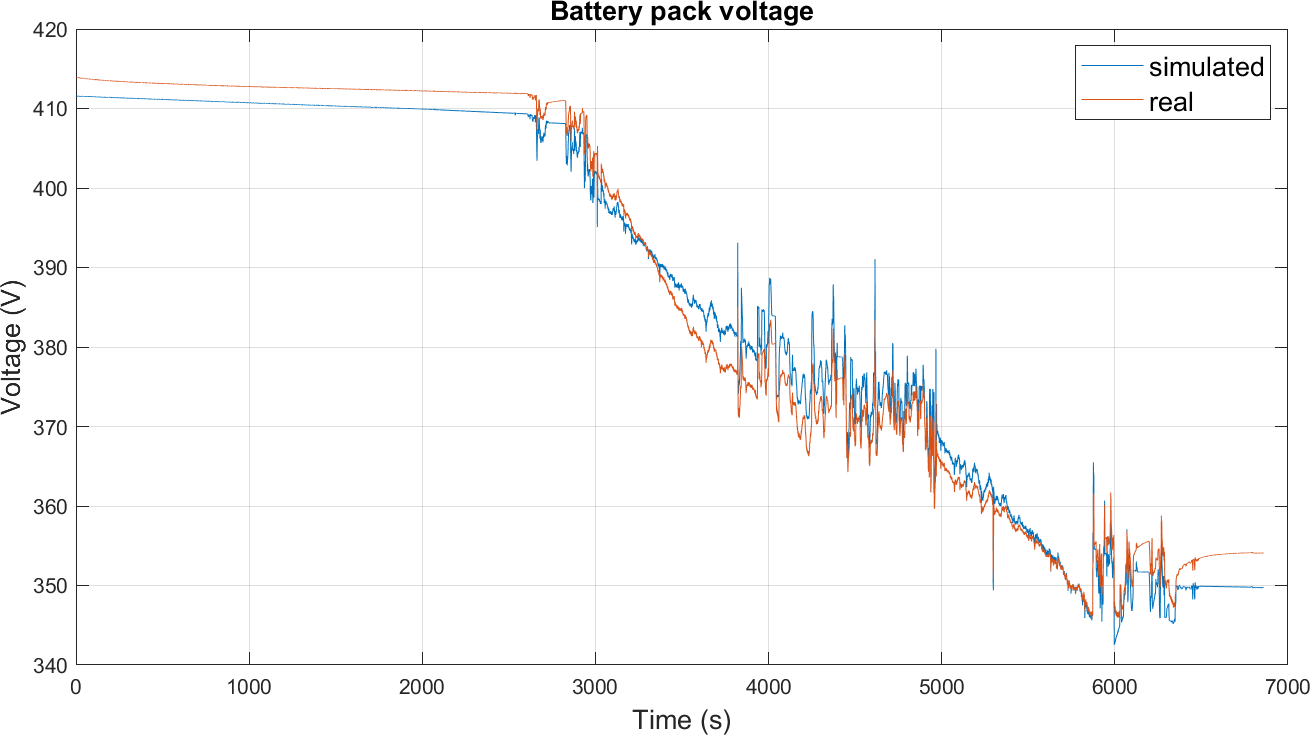
\includegraphics[width=\textwidth]{images/par_est_V_eup}
    \caption{e-up!}
\end{subfigure}

\vspace{20pt}

\begin{subfigure}{\textwidth}
    \centering
    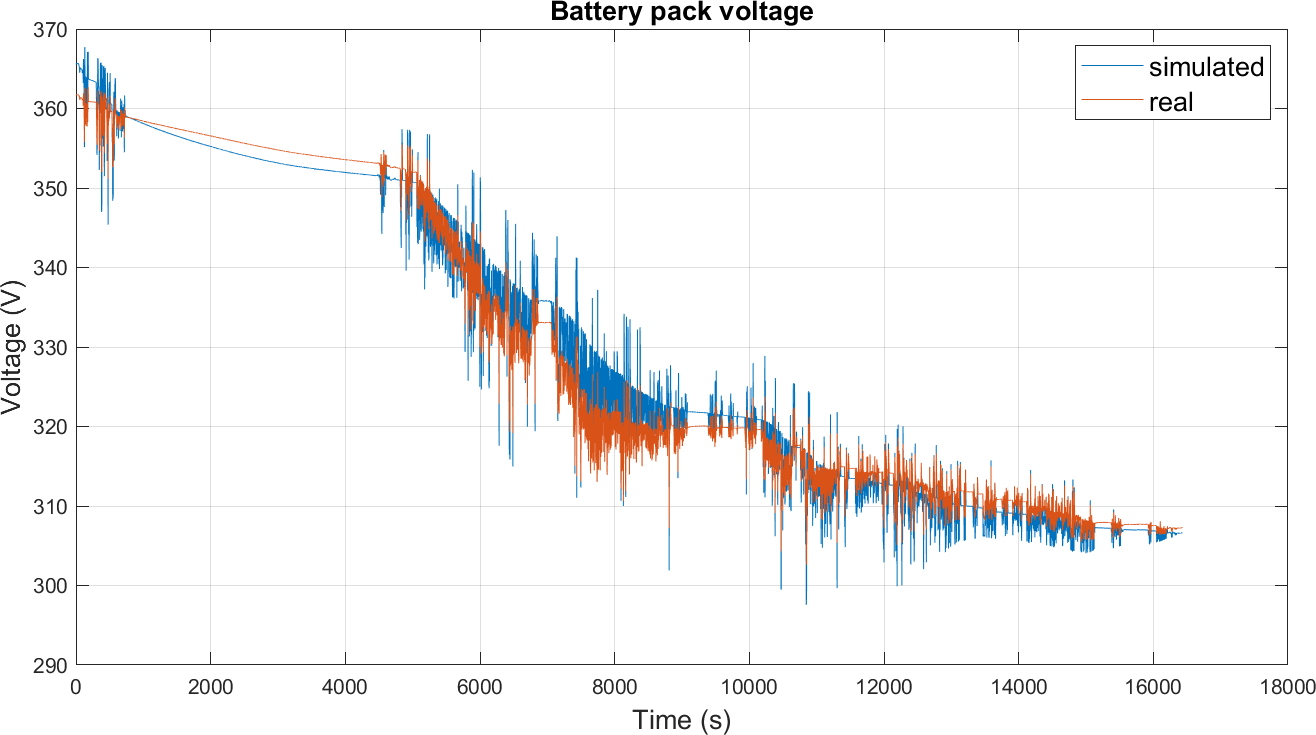
\includegraphics[width=\textwidth]{images/par_est_V_egolf}
    \caption{e-Golf}
\end{subfigure}
\caption[Simulated and real voltage signal after parameter estimation]{Simulated and real voltage signal after parameter estimation}
\label{fig:par_est_comparison_V}
\end{figure}

\begin{figure}[htbp!]
\centering
\begin{subfigure}{\textwidth}
    \centering
    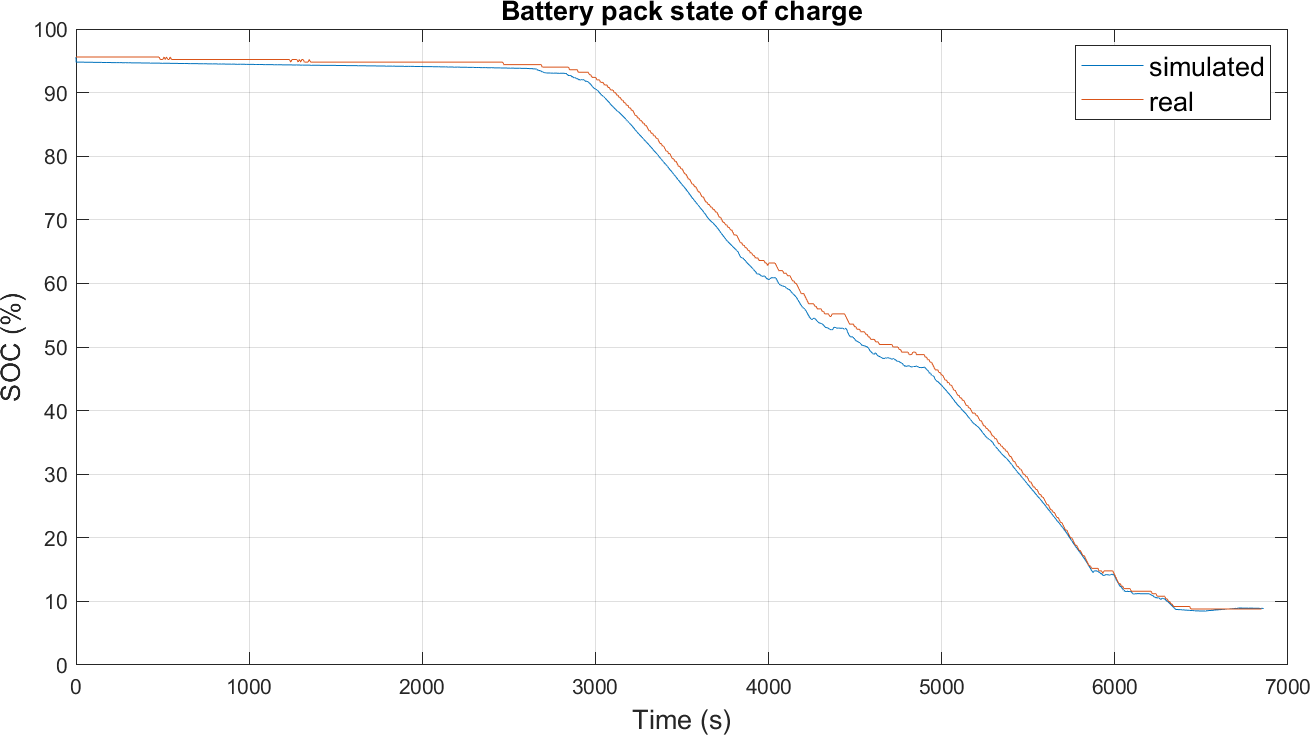
\includegraphics[width=\textwidth]{images/par_est_SOC_eup}
    \caption{e-up!}
\end{subfigure}

\vspace{20pt}

\begin{subfigure}{\textwidth}
    \centering
    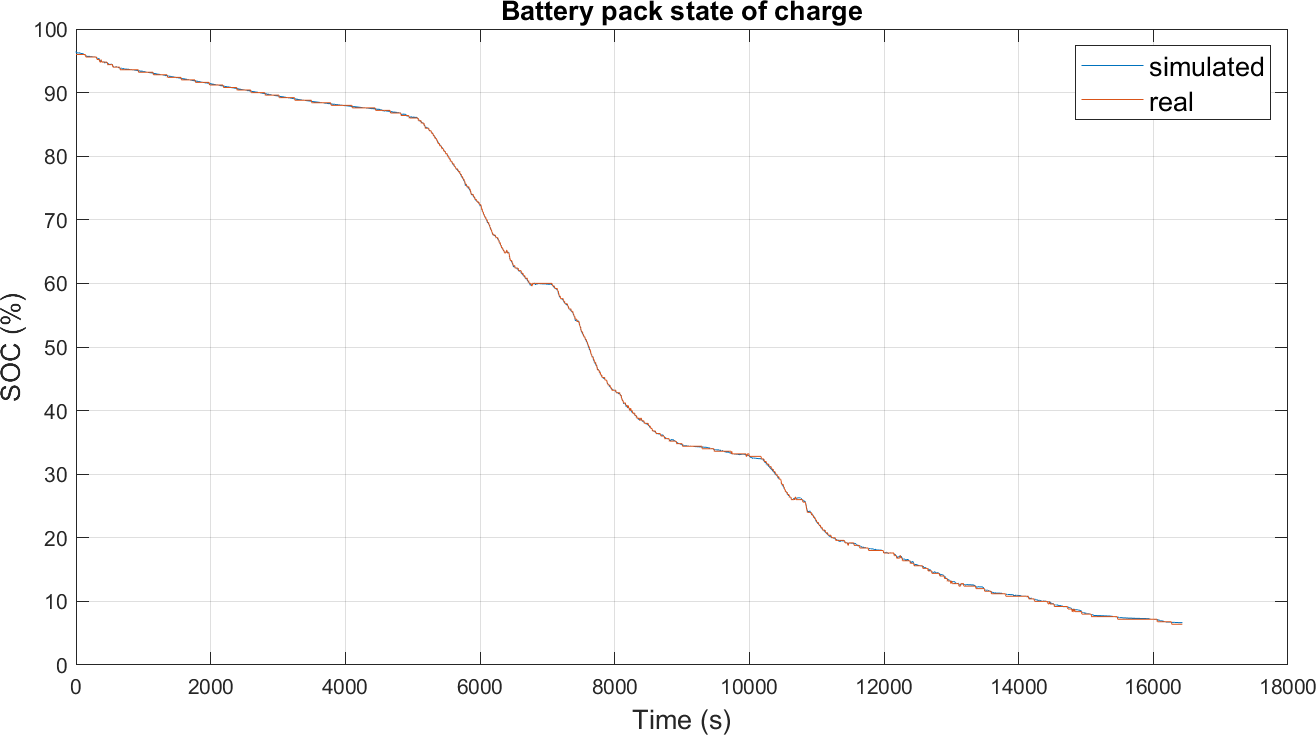
\includegraphics[width=\textwidth]{images/par_est_SOC_egolf}
    \caption{e-Golf}
\end{subfigure}
\caption[Simulated and real SOC signal after parameter estimation]{Simulated and real SOC signal after parameter estimation}
\label{fig:par_est_comparison_SOC}
\end{figure}

As for the thermal model, the thermal resistance and thermal time constant have been estimated by trial and error. Namely, they were initialized to different values for many simulations, and the values for which the deviation between the simulated and real battery temperature was low enough were kept. Fig. \ref{fig:par_est_comparison_T} shows a comparison of the simulated temperature signal versus the experimental (real) one. The deviation between the simulated and real signal is very high at times, but the general trend of the real signal is mimicked successfully. We claim that this behaviour is due to the very low-complexity thermal model that the Simulink battery block implements (as discussed in sec. \ref{sec:known_limitations}).

\begin{figure}[htbp!]
\centering
\begin{subfigure}{\textwidth}
    \centering
    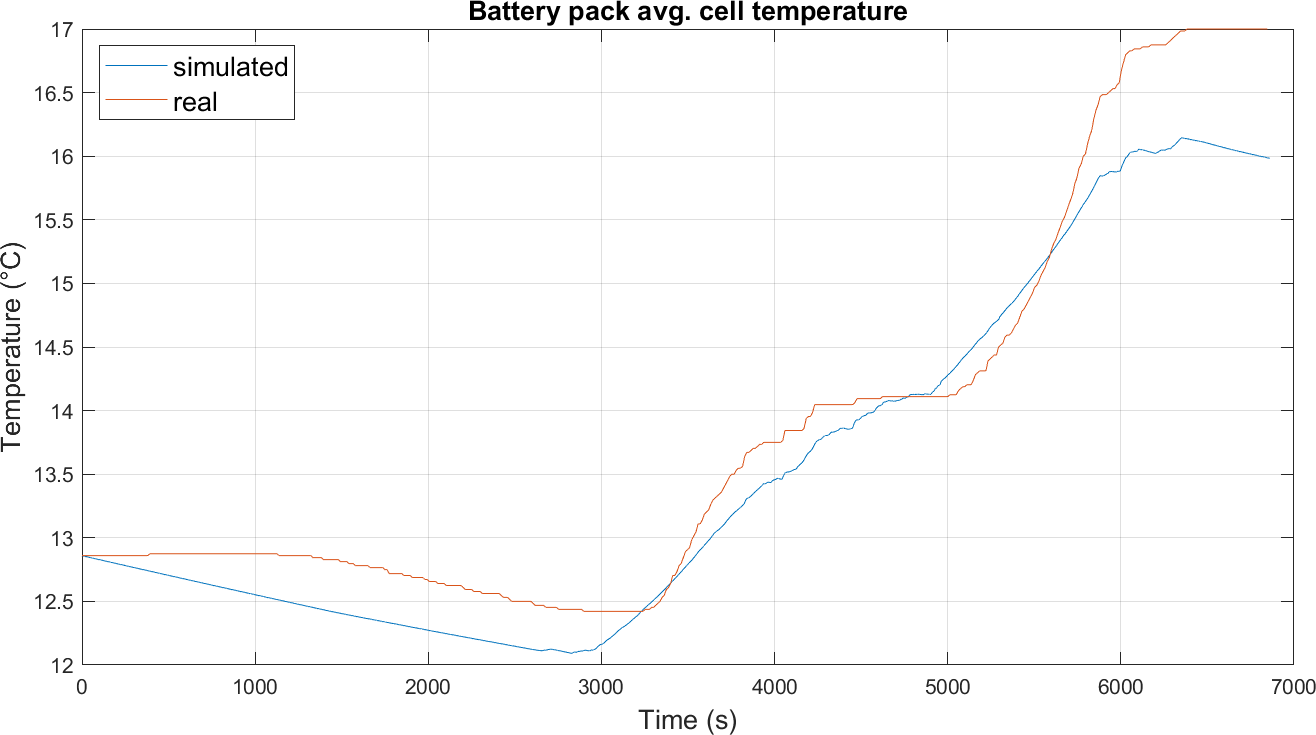
\includegraphics[width=\textwidth]{images/par_est_T_eup}
    \caption{e-up!}
\end{subfigure}

\vspace{20pt}

\begin{subfigure}{\textwidth}
    \centering
    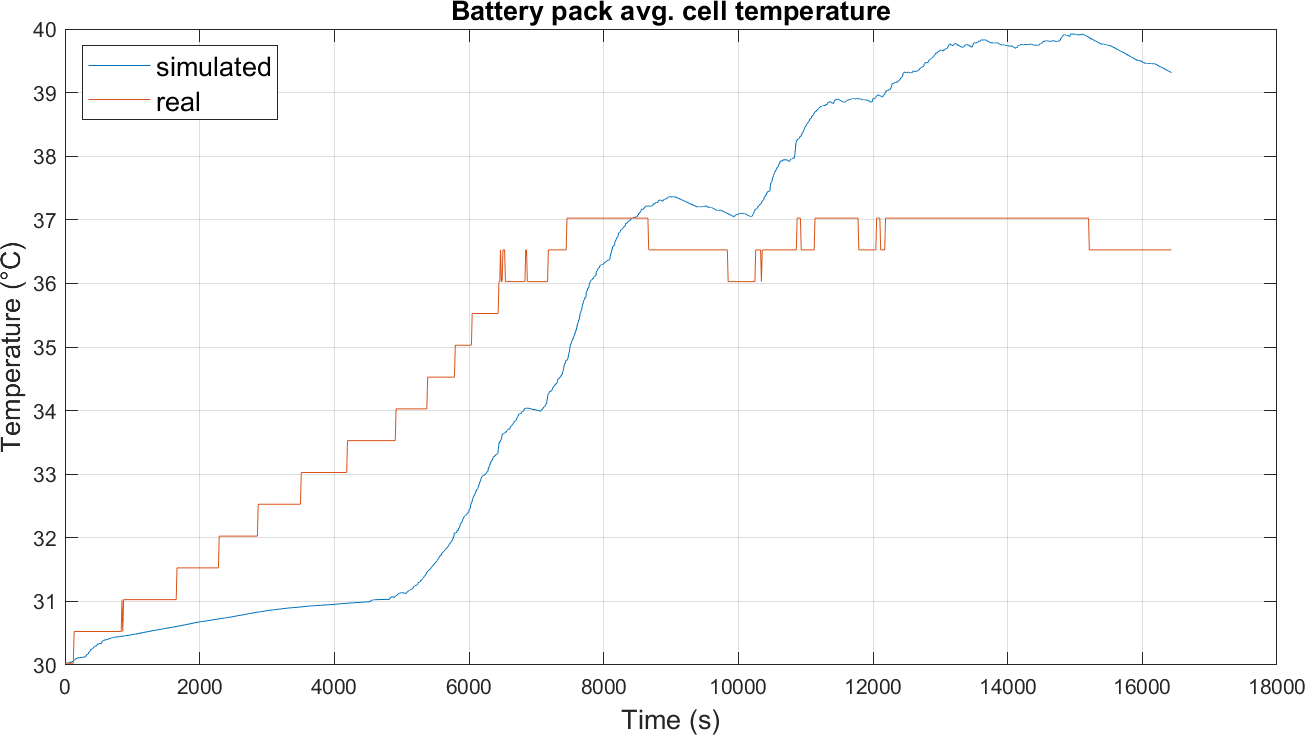
\includegraphics[width=\textwidth]{images/par_est_T_egolf}
    \caption{e-Golf}
\end{subfigure}
\caption{Simulated vs real temperature signal after (manual) parameter estimation}
\label{fig:par_est_comparison_T}
\end{figure}





\section{EFC to SOH conversion}
\label{sec:efc2soh}
As discussed in sec. \ref{sec:soh}, there is no general mathematical relationship between the SOH and the number of EFC. The age of the generic battery model in Simulink can only be set as number of EFC; however, we are interested in expressing the age of the battery pack in terms of SOH.

To overcome this issue, we can set up a simple Simulink simulation which consists in imposing a constant 1C discharge current to the battery block (with an initial SOC of 100\%) and waiting for its complete discharge (SOC = 0\%). Then, the actual capacity of the battery is computed by simply multiplying the magnitude of the imposed discharge current and the ending time of the simulation (in hours). This capacity estimation technique is known as Coulomb counting (sec. \ref{sec:dmb_methods}). Finally, the SOH is obtained by dividing the result of the multiplication by the maximum theoretical capacity of the battery under nominal operating conditions (\texttt{maxCap}).

Since the battery pack aging model is parametrized in the same way for the e-up! and the e-Golf Simulink models, the EFC-to-SOH mapping is unique for the two models. The experiment has been performed 31 times, for EFC values ranging from 0 to 3000 with a step of 100. The resulting mapping is reported graphically in fig. \ref{fig:efc2soh}.

\begin{figure}[hbt!]
    \centering
    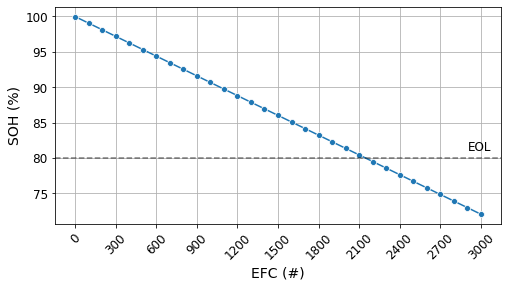
\includegraphics[width=0.75\textwidth]{images/efc2soh}
    \caption[EFC to SOH conversion]{EFC to SOH conversion (linearly interpolated)}
    \label{fig:efc2soh}
\end{figure}

It appears that Simulink's generic battery model is characterized by a linear relationship between EFC and SOH (as opposed to a generic real battery).






\section{Synthetic dataset generation}
\label{sec:ds_gen}
The parametrized EV model can now be used to generate a synthetic dataset of EV monitoring data. To simulate a single driving session, the user must specify a driving cycle, outside temperature [°C] (fixed or as a time series of measurements), initial average battery pack temperature [°C], initial battery pack SOC and battery pack SOH. The monitored signals are: speed [km/h], terminal voltage V [V], current I [A], SOC(\%), average battery internal temperature T [°C]. Additionally, the user can specify a specific \texttt{sampling\_rate} for the monitored signals (default is 0.2 s). Resampling through linear interpolation is performed at the end of each simulation on all the acquired signals according to the specified sampling rate, in order to achieve a common time base for all the signals. The choice of the sampling rate is a trade-off between computation time and signal fidelity: a fast sampling rate may capture high frequency changes in the signals more accurately, at the cost of a higher simulation time.

Since it is infeasible to acquire data for every possible combination of SOH, driving cycle, initial internal and external temperature, we design the following synthetic dataset generation procedure, with the aim of acquiring a minimal but sufficiently representative set of monitoring data in a very wide range of driving conditions:

\begin{algorithm}
\caption{Simulink EV model synthetic dataset generation}
\label{alg:ds_gen}
\begin{algorithmic}[1]
\For{\texttt{efc} $\in$ \texttt{EFC\_LEVELS}}
    \For{\texttt{dc} $\in$ \texttt{DC\_LIST}}
        \State $\text{\texttt{initSOC}} \gets \mathcal{U}(91,96)$
        \State $\text{\texttt{T\_outside}} \gets \mathcal{U}(-5,30)$
        \State $\text{\texttt{initBattTemp}} \gets \mathcal{U}(\text{\texttt{T\_outside}},\text{\texttt{T\_outside}}+5)$
        \State \textbf{simulate} \texttt{dc} in loop until $\text{SOC} < 10$
        \State get simulated signals (speed, V, I, SOC, T)
        \State resample signals every \texttt{sampling\_rate} s
        \State store dataset on disk
    \EndFor
\EndFor
\State concatenate datasets
\end{algorithmic}
\end{algorithm}

where "$\leftarrow\mathcal{U}(a,b)$" is a random extraction from the uniform distribution on $[a,b]$, \texttt{EFC\_LEVELS} is a list of EFC values at which to set the battery block for the simulation and \texttt{DC\_LIST} is a list of drive cycles that we wish to simulate.

To be representative, the synthetic dataset should contain driving session data associated to SOH values ranging from 100\% to 80\% (end of life); therefore we have set \texttt{EFC\_LEVELS} = [0, 100, 200, \dots, 2000] (since EFC = 2000 roughly corresponds to SOH = 80\%). Moreover, to span different driving conditions (city, urban and highway driving\footnote{We can categorize drive cycles in three categories: city (max speed <50 km/h), urban (max speed <90 km/h), highway (max speed >90 km/h).}), 12 standard drive cycles \cite{drive_cycles} have been included in \texttt{DC\_LIST}; they are listed in tab. \ref{tab:dc_list}. Additionally, we have also included three driving cycles (2x highway, 1x urban) extracted from the e-up! real dataset (chap. \ref{sec:aviloo_ds}), for a total of 15 drive cycles.

\begin{table}[htb!]
\centering
\begin{tabular}[t]{cc}
\toprule
Drive cycle name & Type\\
\midrule
Artemis Urban & city\\
Artemis Rural Road & urban\\
Artemis Motorway 130 kmph & highway\\
ECE R15 & city\\
EUDC & highway\\
FTP72 & urban\\
IM240 & urban\\
J1015 & city\\
LA92 & urban\\
NYCC & city\\
UDDS & urban\\
US06 & highway\\
\bottomrule
\end{tabular}
\caption[Selected standard drive cycles]{Standard drive cycles included in \texttt{DC\_LIST}.}
\label{tab:dc_list}
\end{table}

The dataset generation procedure has been run once for each EV model. Each of the two resulting datasets consists of a combination of 315 driving sessions, each associated to a specific (SOH, drive cycle) combination. There is no invalid or missing data. Before using these two synthetically generated datasets, they are further cleaned and preprocessed as explained in sec. \ref{sec:ds_preprocessing}.